\section[Ход работы]{ХОД РАБОТЫ}

\subsection{Описание предметной области}

В качестве предметной области данной расчетной работы выберем
описание и автоматизацию учета данных бизнес-процессов спортивного магазина,
занимающегося реализацией экипировки для настольного тенниса.
Будем рассматривать следующие объекты предметной области:
\begin{itemize}
\item товар (ракетки, основания, накладки и шарики);
\item производители товара;
\item поставщики товара.
\end{itemize}

Определим следующие бизнес-процессы предметной области:
\begin{itemize}
\item поступление товара;
\item реализация товара.
\end{itemize}

Перечислим задачи, решаемые разрабатываемой системой:
\begin{itemize}
\item учет поступления и реализации товара;
\item предоставление информации на основе накопленных данных.
\end{itemize}

\subsection{Создание перечислений}

Создание перечислений производится с помощью раздела <<Перечисления>>
панели <<Конфигурация>> режима <<Конфигуратор>>.
Для создания перечисления необходимо, щелкнув правой кнопкой мыши по этому
разделу, выбрать пункт <<Добавить>>. Далее в появившемся окне
следует определить имя и синоним перечисления.
После этого в разделе <<Данные>> необходимо определить возможные значения
создаваемего перечисления.

В силу специфики предметной области удобно использовать следующие
перечисления для определения множества значений свойств товаров:
\begin{itemize}
\item <<КлассРакетки>> со значениями
  <<S1>> (синоним: <<*>>),
  <<S2>> (синоним: <<**>>),
  <<S3>> (синоним: <<***>>),
  <<S4>> (синоним: <<****>>),
  <<S5>> (синоним: <<*****>>);
\item <<КлассОснования>> со значениями
  <<OFFplus>> (синоним: <<OFF+>>),
  <<OFF>> (синоним: <<OFF>>),
  <<OFFminus>> (синоним: <<OFF->>),
  <<ALL>> (синоним: <<ALL>>),
  <<DEFplus>> (синоним: <<DEF+>>),
  <<DEF>> (синоним: <<DEF>>),
  <<DEFminus>> (синоним: <<DEF->>);
\item <<КлассШарика>> со значениями
  <<S1>> (синоним: <<*>>),
  <<S2>> (синоним: <<**>>),
  <<S3>> (синоним: <<***>>);
\item <<ЦветШарика>> со значениями
  <<Белый>> и
  <<Оранжевый>>.
\end{itemize}

На рисунке~\ref{fig:enum} приведены
значения перечисления <<КлассРакетки>> в интерфейсе конфигуратора
СКД 1C:Предприятие.

\begin{figure}[h!]
  \centering
  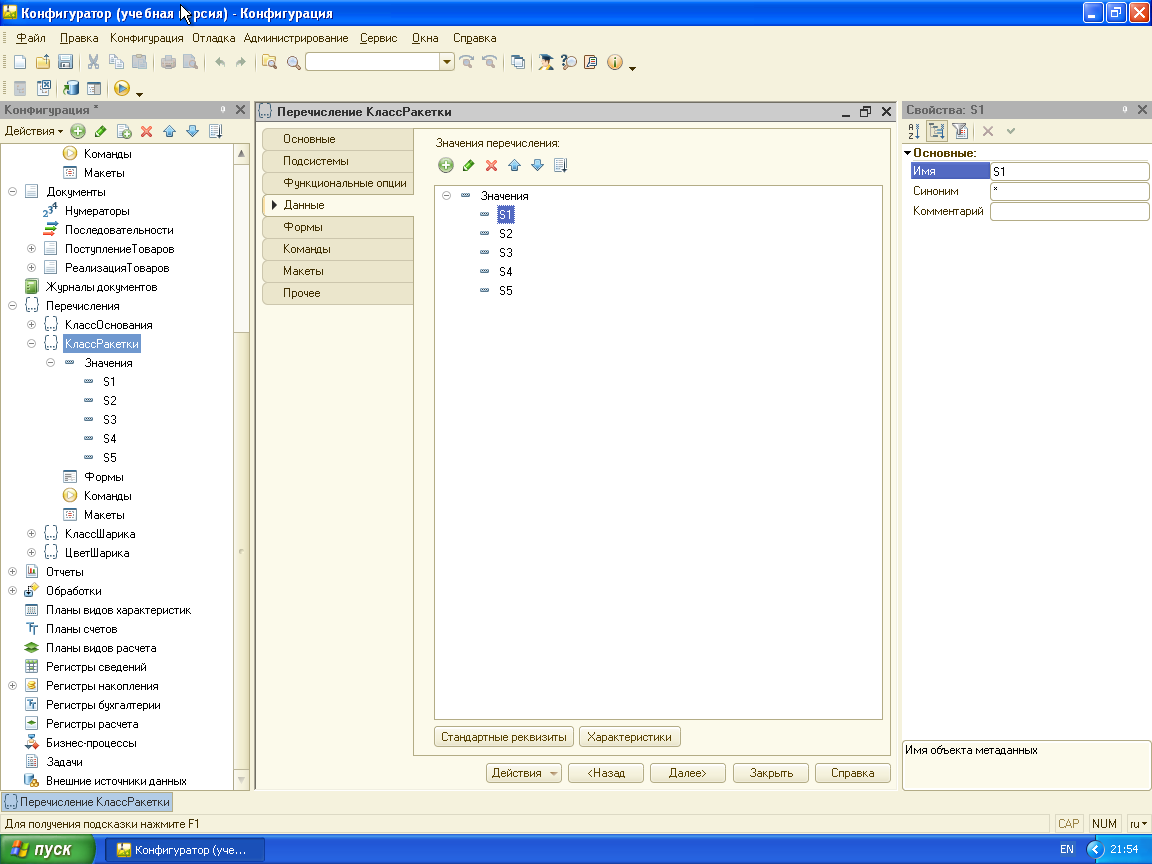
\includegraphics[width=150mm]{pic/enum}
  \caption{Значения перечисления <<КлассРакетки>>}
  \label{fig:enum}
\end{figure}

Созданные перечисления призваны сэкономить время и снизить количество
ошибок при заполнении справочников.

\subsection{Создание справочников}

Создание справочников производится с помощью раздела <<Справочники>>
панели <<Конфигурация>> режима <<Конфигуратор>>.
Для создания справочника необходимо, щелкнув правой кнопкой мыши по этому
разделу, выбрать пункт <<Добавить>>. Далее в появившемся окне
следует определить имя и синоним справочника.
После этого в разделе <<Данные>> необходимо определить структуру
хранимых данных путем добавления и указания свойств реквизитов
и табличных частей.

В разрабатываемой информационной системе справочники соответствуют
объектам предметной области: <<Производители>>, <<Поставщики>>,
<<Ракетки>>, <<Основания>>, <<Накладки>>, <<Шарики>>.

Структура справочника <<Производители>>:
\begin{itemize}
\item поле <<Наименование>>, вводимое вручную (длина: 25);
\item реквизит <<Страна>> (тип: строка, длина: 50);
\item реквизит <<Описание>> (тип: строка, длина: неограниченная).
\end{itemize}

Структура справочника <<Поставщики>>:
\begin{itemize}
\item поле <<Наименование>>, вводимое вручную (длина: 250);
\item реквизит <<ЮридическийАдрес>> (тип: строка, длина: 50);
\item табличная часть <<КонтактныеЛица>>, содержащая поля
  <<ФИО>> (тип: строка, длина: 50),
  <<Должность>> (тип: строка, длина: 50) и
  <<Номер телефона>> (тип: строка, длина: 20).
\end{itemize}

На рисунке~\ref{fig:sprav_postav} приведена
структура справочника <<Поставщики>> в интерфейсе конфигуратора
СКД 1C:Предприятие.

\begin{figure}[h!]
  \centering
  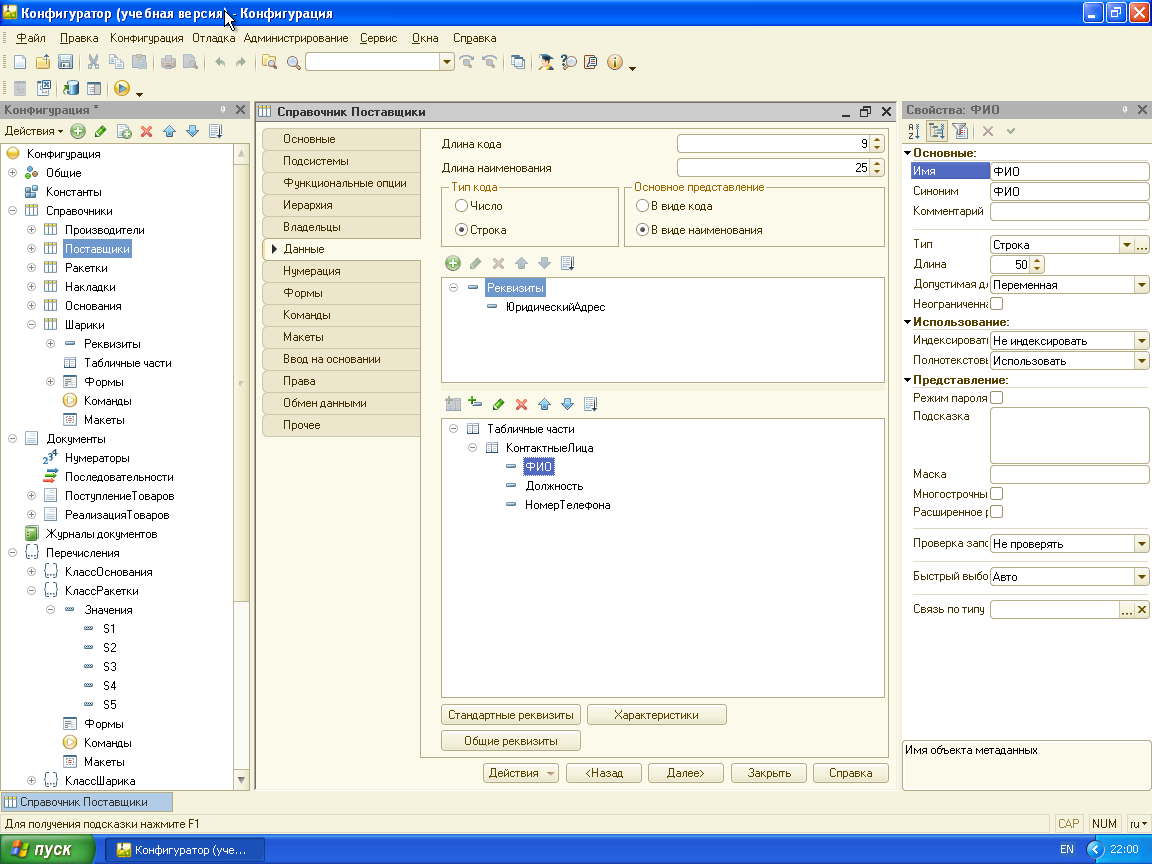
\includegraphics[width=150mm]{pic/sprav_postav}
  \caption{Структура справочника <<Поставщики>>}
  \label{fig:sprav_postav}
\end{figure}

Структура справочника <<Ракетки>>:
\begin{itemize}
\item поле <<Наименование>>, формируемое автоматически (длина: 25);
\item реквизит <<Производитель>> (тип: <<СправочникСсылка.Производи-тели>>);
\item реквизит <<Модель>> (тип: строка, длина: 25);
\item реквизит <<Класс>> (тип: <<ПеречислениеСсылка.КлассРакетки>>);
\item реквизит <<Вес>> (тип: число).
\end{itemize}

Для того, чтобы значение поля <<Наименование>> справочника <<Ракетки>>
формировалось на основании значения реквизитов <<Производитель>> и <<Модель>>
автоматически, создадим форму ввода данных <<ВводДанных>>,
удалим с неё элемент ввода наименования, как показано на
рисунке~\ref{fig:sprav_auto_name} и назначим обработчики событий
<<ПроизводительПриИзменении>> и <<МодельПриИзменении>>,
как показано на рисунке~\ref{fig:sprav_auto_name_module}.

\begin{figure}[h!]
  \centering
  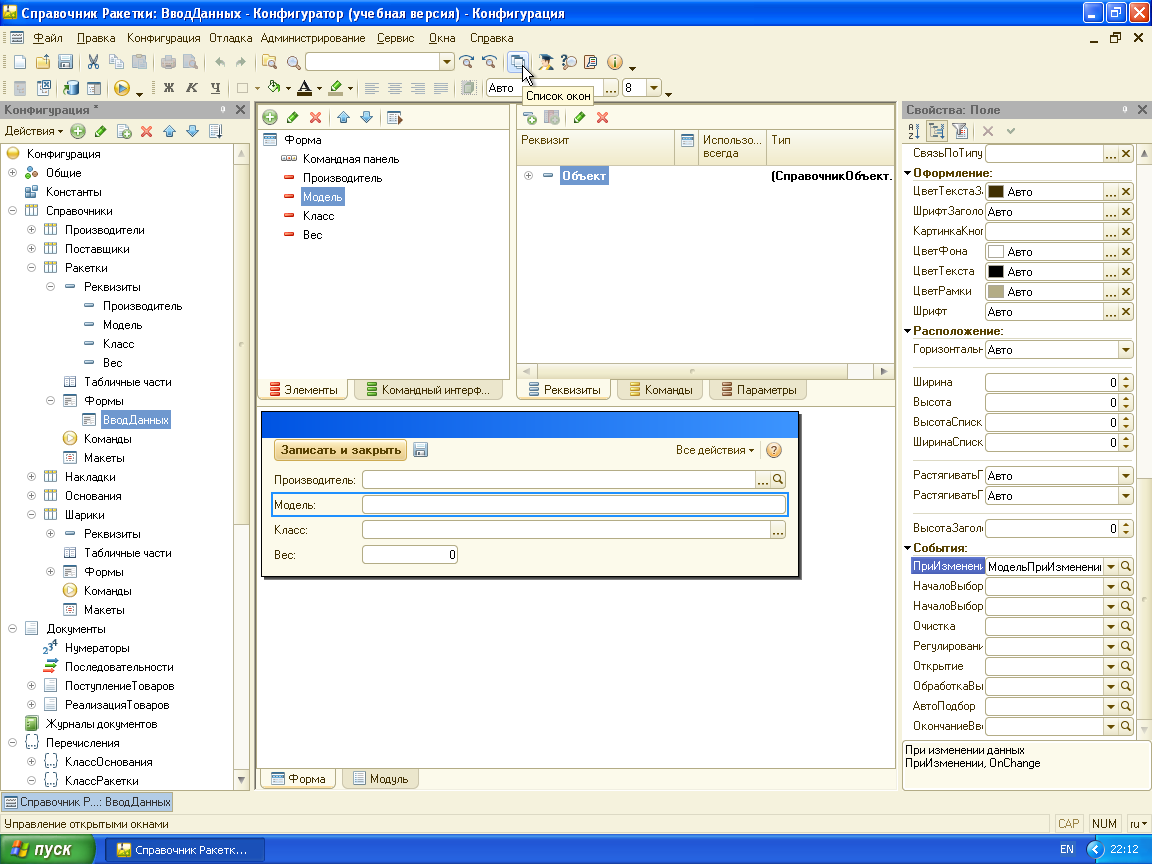
\includegraphics[width=150mm]{pic/sprav_auto_name}
  \caption{Модифицированная форма ввода данных \\ справочника <<Ракетки>>}
  \label{fig:sprav_auto_name}
\end{figure}

\begin{figure}[h!]
  \centering
  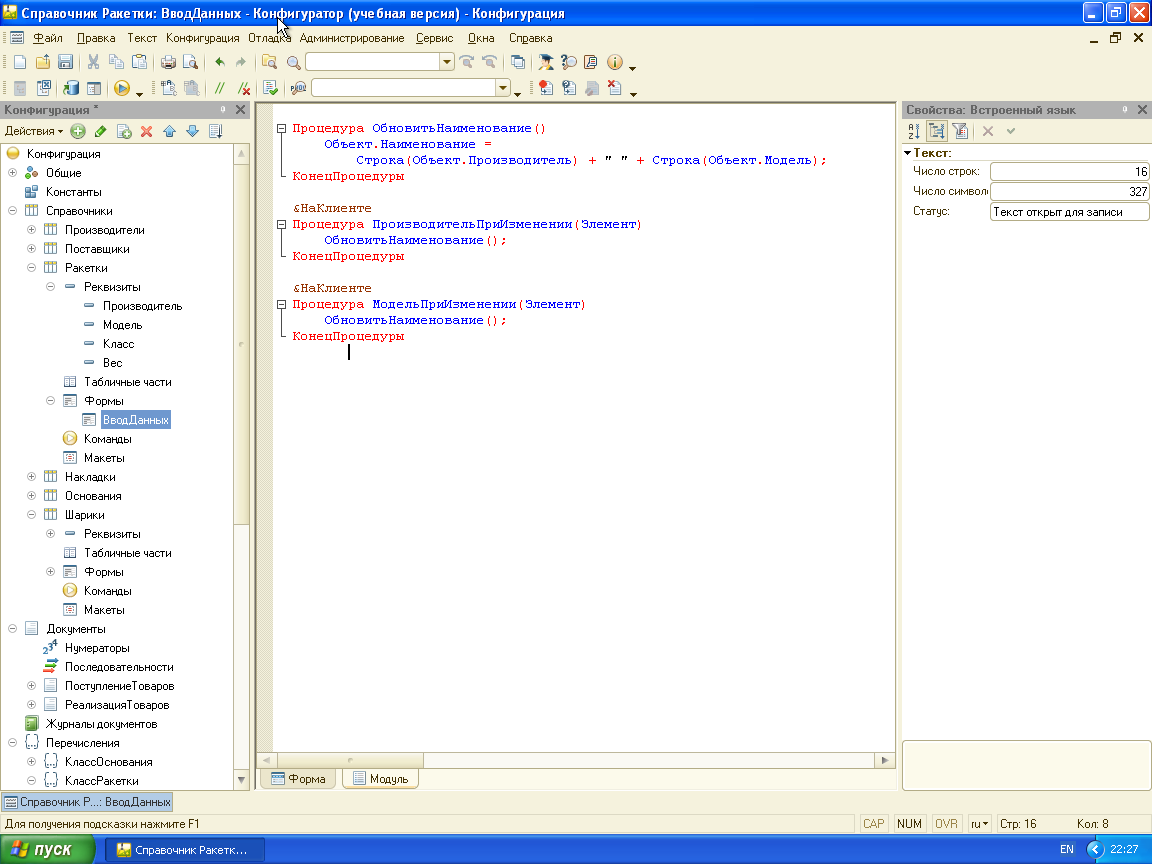
\includegraphics[width=130mm]{pic/sprav_auto_name_module}
  \caption{Обработчики событий формы ввода данных \\ справочника <<Ракетки>>}
  \label{fig:sprav_auto_name_module}
\end{figure}

Структура справочника <<Основания>>:
\begin{itemize}
\item поле <<Наименование>>, формируемое автоматически (длина: 25);
\item реквизит <<Производитель>> (тип: <<СправочникСсылка.Производи-тели>>);
\item реквизит <<Модель>> (тип: строка, длина: 50);
\item реквизит <<Класс>> (тип: <<ПеречислениеСсылка.КлассОснования>>);
\item реквизит <<Вес>> (тип: число).
\end{itemize}

Структура справочника <<Накладки>>:
\begin{itemize}
\item поле <<Наименование>>, формируемое автоматически (длина: 25);
\item реквизит <<Производитель>> (тип: <<СправочникСсылка.Производи-тели>>);
\item реквизит <<Модель>> (тип: строка, длина: 50);
\item реквизиты <<Скорость>>, <<Вращение>> и <<Контроль>>
  (тип: число, минимальное: 0, максимальное: 100).
\end{itemize}

Структура справочника <<Шарики>>:
\begin{itemize}
\item поле <<Наименование>>, формируемое автоматически (длина: 25);
\item реквизит <<Производитель>> (тип: <<СправочникСсылка.Производи-тели>>);
\item реквизит <<Класс>> (тип: <<ПеречислениеСсылка.КлассШарика>>);
\item реквизит <<Цвет>> (тип: <<ПеречислениеСсылка.Цвет>>).
\end{itemize}

Значение поля <<Наименование>> справочников <<Основания>>, <<Накладки>> и <<Шарики>>
формируется аналогично.

\subsection{Создание документов}

Создание документов производится с помощью раздела <<Документы>>
панели <<Конфигурация>> режима <<Конфигуратор>>.
Для создания документа необходимо, щелкнув правой кнопкой мыши по этому
разделу, выбрать пункт <<Добавить>>. Далее в появившемся окне
следует определить имя и синоним документа.
После этого в разделе <<Данные>> необходимо определить структуру
хранимых данных путем добавления и указания свойств реквизитов
и табличных частей.

В разрабатываемой информационной системе документы используются для
регистрации фактов поступления и реализации товаров.

%% Поступление товаров
Структура документа <<ПоступлениеТоваров>>:
\begin{itemize}
\item реквизит <<Поставщик>> (тип: СправочникСсылка.Поставщики);
\item реквизит <<ОбщаяСтоимость>> (тип: число, длина: 10, неотрицательное);
\item табличная часть <<ПереченьТоваров>>, содержащая поля
  <<Наименование>> (тип: составной(%
  СправочникСсылка.Ракетки,
  СправочникСсылка.Основания,
  СправочникСсылка.Накладки,
  СправочникСсылка.Шарики)),
  <<Цена>> (тип: число, длина: 10, неотрицательное),
  <<Количество>> (тип: число, длина: 10, неотрицательное),
  <<Стоимость>> (тип: число, длина: 10, неотрицательное).
\end{itemize}

Для указания составного типа данных для некоторого реквизита необходимо в
редакторе поля <<Тип>> установить параметр <<Составной тип данных>>,
как показано на рисунке~\ref{fig:complex_type}.

\begin{figure}[h!]
  \centering
  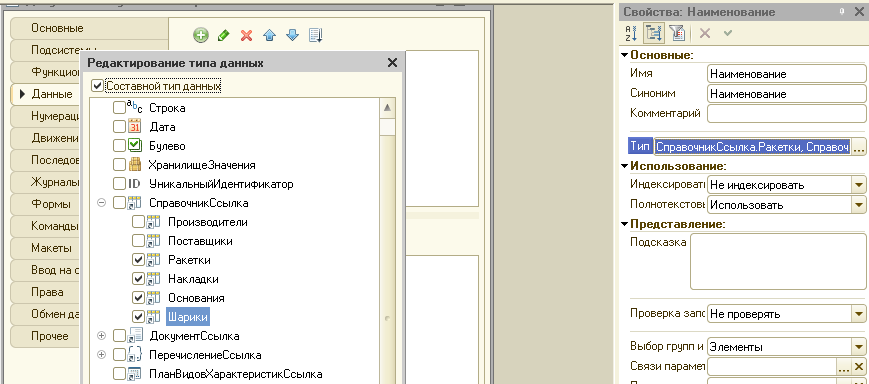
\includegraphics[width=150mm]{pic/complex_type}
  \caption{Выбор составного типа данных}
  \label{fig:complex_type}
\end{figure}

На рисунке~\ref{fig:doc_input} приведена
структура документа <<ПоступлениеТоваров>> в интерфейсе конфигуратора
СКД 1C:Предприятие.

\begin{figure}[h!]
  \centering
  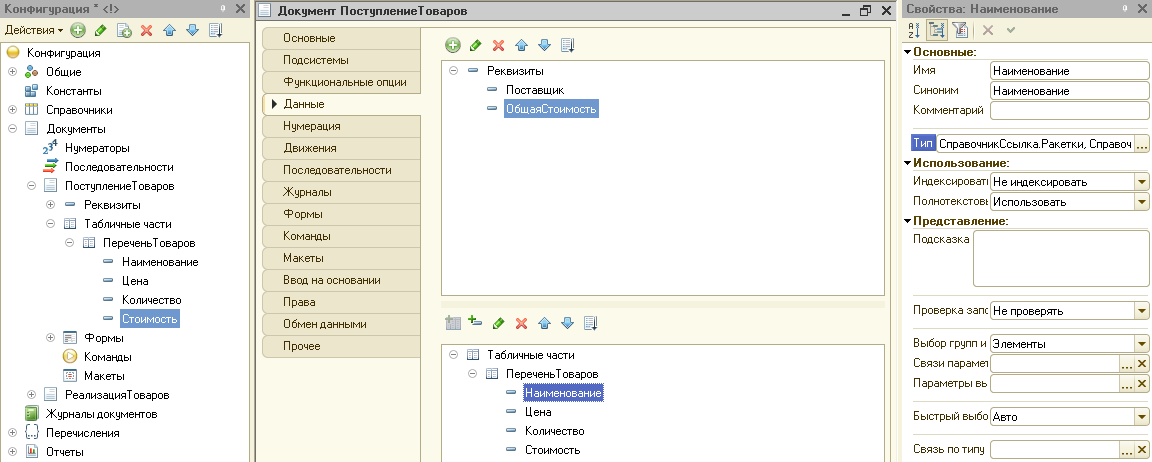
\includegraphics[width=150mm]{pic/doc_input}
  \caption{Структура документа <<ПоступлениеТоваров>>}
  \label{fig:doc_input}
\end{figure}

Для того, чтобы при вводе цены и количества товара автоматически
рассчитывалась его стоимость, а также рассчитывалась общая стоимость
поставки, назначим обработчики событий
<<ПриОткрытии>>,
<<ПереченьТоваровЦенаПриИзменении>>,
<<ПереченьТоваровКоличествоПриИзменении>>,
<<ПереченьТоваровПослеУдаления>>
формы документа, как показано на рисунке~\ref{fig:doc_input_module}.

\begin{figure}[h!]
  \centering
  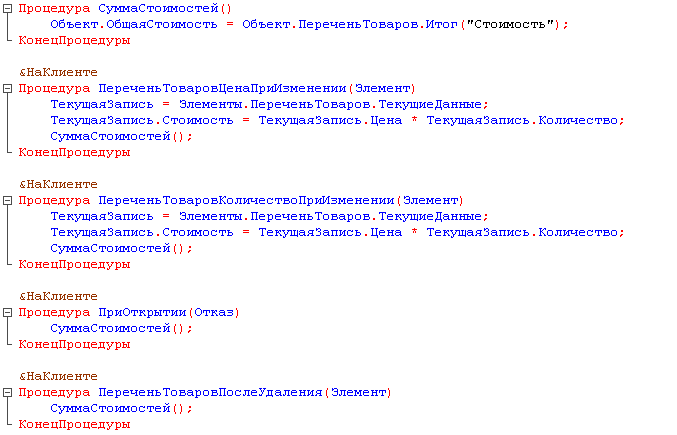
\includegraphics[width=130mm]{pic/doc_input_module}
  \caption{Обработчики событий формы ввода данных \\
    документа <<ПоступлениеТоваров>>}
  \label{fig:doc_input_module}
\end{figure}

%% Реализация товаров
Структура документа <<РеализацияТоваров>>:
\begin{itemize}
\item реквизит <<Поставщик>> (тип: СправочникСсылка.Поставщики);
\item реквизит <<ОбщаяСтоимость>> (тип: число, длина: 10, неотрицательное);
\item реквизит <<РазмерСкидки>> (тип: число, длина: 10, неотрицательное);
\item реквизит <<ИтоговаяСтоимость>> (тип: число, длина: 10, неотрицательное);
\item реквизит <<ПроцентСкидки>> (тип: число, длина: 2, неотрицательное);
\item табличная часть <<ПереченьТоваров>>, содержащая поля
  <<Наименование>> (тип: составной(%
  СправочникСсылка.Ракетки,
  СправочникСсылка.Основания,
  СправочникСсылка.Накладки,
  СправочникСсылка.Шарики)),
  <<Цена>> (тип: число, длина: 10, неотрицательное),
  <<Количество>> (тип: число, длина: 10, неотрицательное),
  <<Стоимость>> (тип: число, длина: 10, неотрицательное).
\end{itemize}

На рисунке~\ref{fig:doc_output} приведена
структура документа <<РеализацияТоваров>> в интерфейсе конфигуратора
СКД 1C:Предприятие.

\begin{figure}[h!]
  \centering
  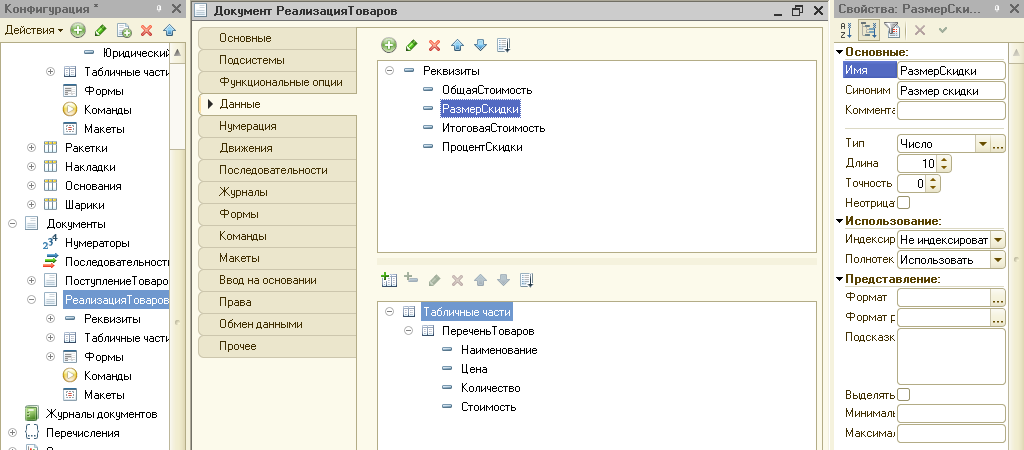
\includegraphics[width=150mm]{pic/doc_output}
  \caption{Структура документа <<РеализацияТоваров>>}
  \label{fig:doc_output}
\end{figure}

Для того, чтобы при вводе цены и количества и размера скидки на товар автоматически
рассчитывалась его стоимость и общая стоимость
поставки, назначим обработчики событий
<<ПриОткрытии>>,
<<ПереченьТоваровЦенаПриИзменении>>,
<<ПереченьТоваровКоличествоПриИзменении>>,
<<ПереченьТоваровПослеУдаления>>
формы документа, как показано на рисунке~\ref{fig:doc_output_module}.

\begin{figure}[h!]
  \centering
  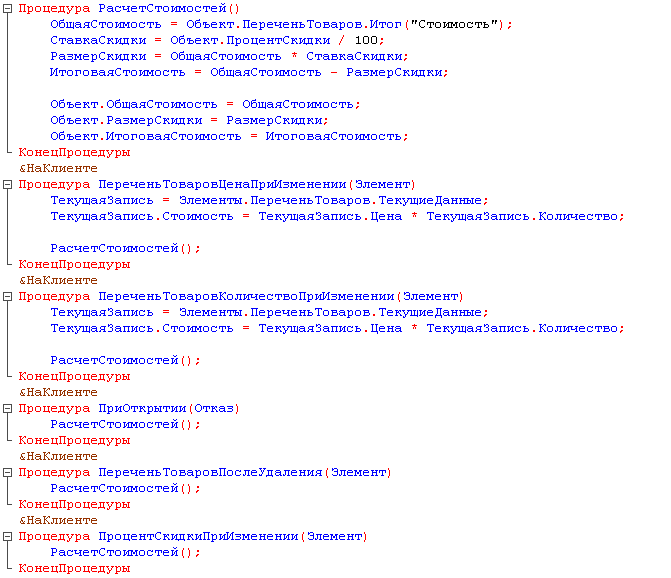
\includegraphics[width=130mm]{pic/doc_output_module}
  \caption{Обработчики событий формы ввода данных \\
    документа <<РеализацияТоваров>>}
  \label{fig:doc_output_module}
\end{figure}

\pagebreak

\subsection{Создание регистра накопления}

Создание регистров накопления производится с помощью раздела
<<Регистры накопления>> панели <<Конфигурация>> режима <<Конфигуратор>>.
Для создания регистра накопления необходимо,
щелкнув правой кнопкой мыши по этому
разделу, выбрать пункт <<Добавить>>. Далее в появившемся окне
следует определить имя и синоним регистра.
После этого в разделе <<Данные>> необходимо определить структуру
хранимых данных путем добавления и указания свойств измерений и ресурсов.

Для регистрации изменения количества и стоимости имеющегося товара
создадим регистр накопления <<КоличествоТовара>> с измерениями
<<Поставщик>> (тип: СправочникСсылка.Поставщики),
<<Товар>> (составной тип: составной(%
  СправочникСсылка.Ракетки,
  СправочникСсылка.Основания,
  СправочникСсылка.Накладки,
  СправочникСсылка.Шарики)
и ресурсами
<<Количество>> (тип: число, длина: 10),
<<Стоимость>> (тип: число, длина: 10),
как показано на рисунке~\ref{fig:reg_structure}.

\begin{figure}[h!]
  \centering
  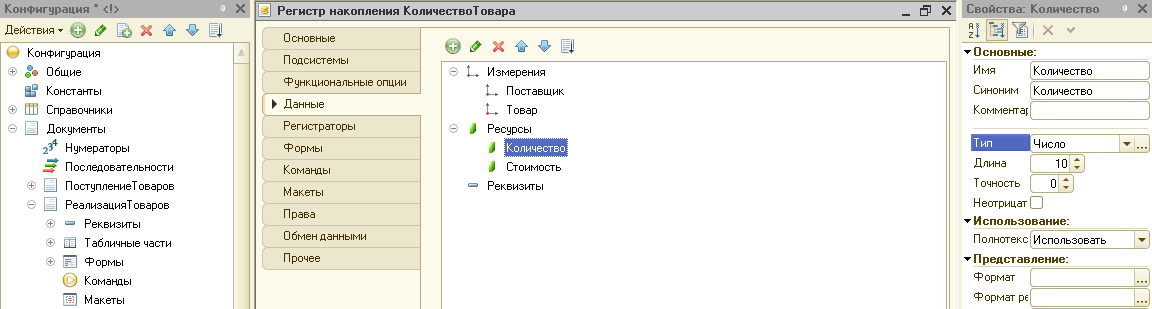
\includegraphics[width=150mm]{pic/reg_structure}
  \caption{Структура регистра накопления <<КоличествоТовара>>}
  \label{fig:reg_structure}
\end{figure}

Для данного регистра укажем документы-регистраторы:
<<ПоступлениеТоваров>> (приход) и
<<РеализацияТоваров>> (расход).

Это можно сделать с помощью конструктора движения регистров,
расположенного на вкладке <<Движения>> свойств документа,
как показано на рисунках~\ref{fig:reg_doc_input},~\ref{fig:reg_doc_output}.

\begin{figure}[h!]
  \centering
  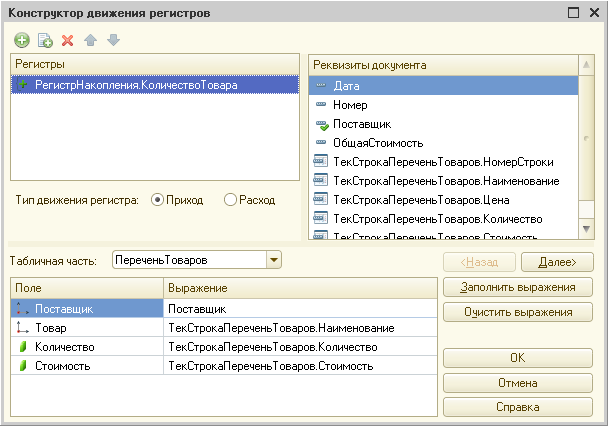
\includegraphics[width=130mm]{pic/reg_doc_input}
  \caption{Параметры регистрации движения документа <<ПоступлениеТоваров>>}
  \label{fig:reg_doc_input}
\end{figure}

\begin{figure}[h!]
  \centering
  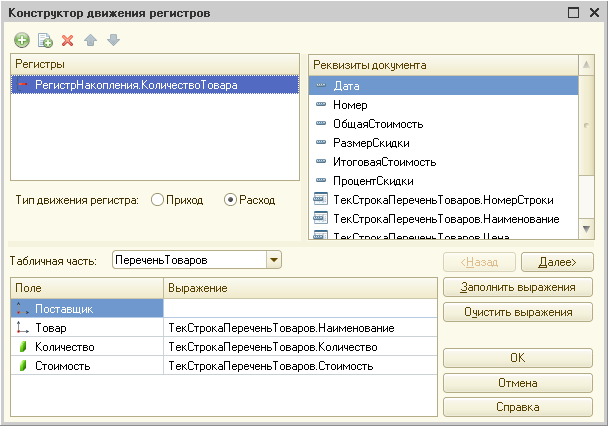
\includegraphics[width=130mm]{pic/reg_doc_output}
  \caption{Параметры регистрации движения документа <<РеализацияТоваров>>}
  \label{fig:reg_doc_output}
\end{figure}

\pagebreak

\subsection{Создание отчетов}

Создание отчетов производится с помощью раздела
<<Отчеты>> панели <<Конфигурация>> режима <<Конфигуратор>>.
Для создания отчета необходимо,
щелкнув правой кнопкой мыши по этому
разделу, выбрать пункт <<Добавить>>. Далее в появившемся окне
следует определить имя и синоним отчета.

Для настройки набора и способа отображения данных в
автоматическом режиме будем использовать
мастер редактирования схемы компоновки данных,
запуск которого производится нажатием кнопки
<<Открыть схему компоновки данных>>, расположенной
на вкладке <<Основные>> окна свойств отчета.

Для выбора данных, отображаемых в отчете, будем использовать
конструктор запроса, запуск которого производится нажатием кнопки
<<Конструктор запроса...>>, расположенной
на вкладке <<Наборы данных>> окна
мастера редактирования схемы компоновки данных отчета.

Для настройки способа отображения данных в отчете будем использовать
конструктор настроек отчета, запуск которого производится нажатием кнопки
<<Конструктор настроек>>, расположенной
на вкладке <<Настройки>> окна
мастера редактирования схемы компоновки данных отчета.

%% Поступления товаров
Создадим отчет о поступлениях товаров,
содержащий данные о поступивших товарах, их количествах и стоимости,
сгруппированные по поставщику.
Для этого в режиме конфигуратора СКД 1С:Предприятие создадим отчет
<<ОтчетПоПоступлениюТоваров>>, с помощью конструктора запросов
определим набор данных, извлекаемых из информационной системы:
<<КоличествоТовараОстаткиИОбороты.Поставщик>>,
<<КоличествоТовараОстаткиИОбороты.Товар>>,
<<КоличествоТовараОстаткиИОбороты.КоличествоПриход>>,
<<КоличествоТовараОстаткиИОбороты.СтоимостьПриход>>,
как показано на рисунке~\ref{fig:report_input_query}.

Схема компоновки данных отчета примет вид,
показанный на рисунке~\ref{fig:report_input_scheme}.

\pagebreak

\begin{figure}[h!]
  \centering
  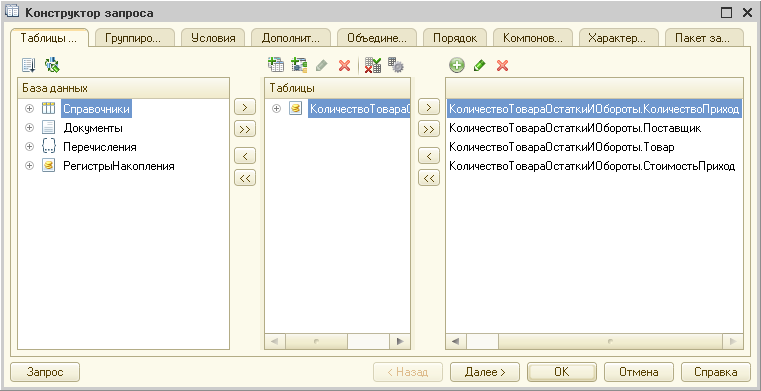
\includegraphics[width=150mm]{pic/report_input_query}
  \caption{Конструктор запросов отчета \\ <<ОтчетПоПоступлениюТоваров>>}
  \label{fig:report_input_query}
\end{figure}

\begin{figure}[h!]
  \centering
  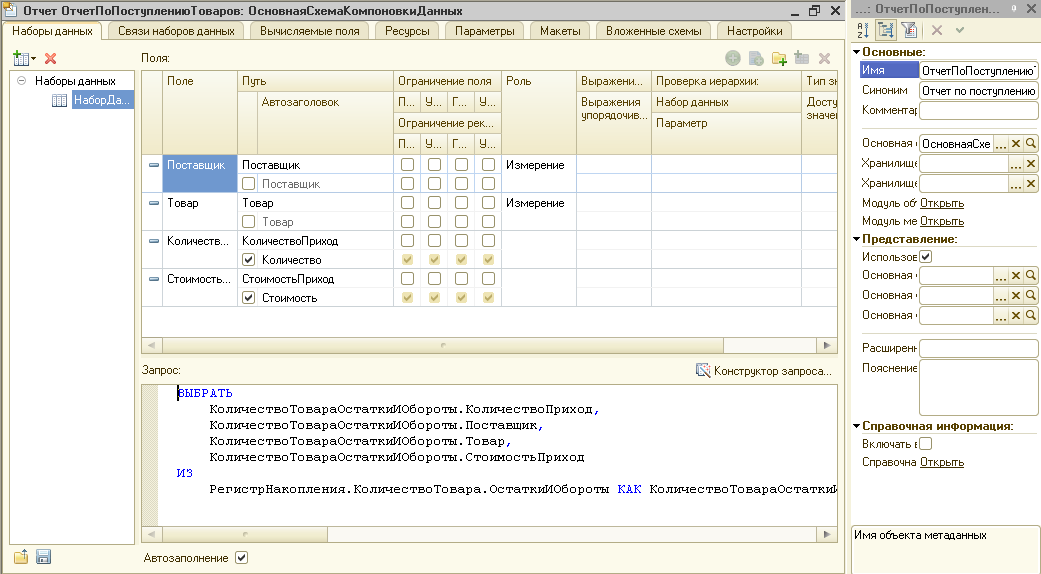
\includegraphics[width=150mm]{pic/report_input_scheme}
  \caption{Схема компоновки данных отчета \\ <<ОтчетПоПоступлениюТоваров>>}
  \label{fig:report_input_scheme}
\end{figure}

\pagebreak

С помощью конструктора настроек отчета выберем желаемый способ отображения
отчета:
\begin{itemize}
\item тип отчета: список;
\item отображаемые поля: <<Поставщик>>, <<Товар>>,
  <<КоличествоПриход>>, <<СтоимостьПриход>>;
\item поля группировки: <<Поставщик>>;
\item поля упорядочивания:
  <<Поставщик>> (по возрастанию),
  <<Товар>> (по возрастанию).
\end{itemize}

Пример разработанного отчета приведен на рисунке~\ref{fig:report_input}.

\begin{figure}[h!]
  \centering
  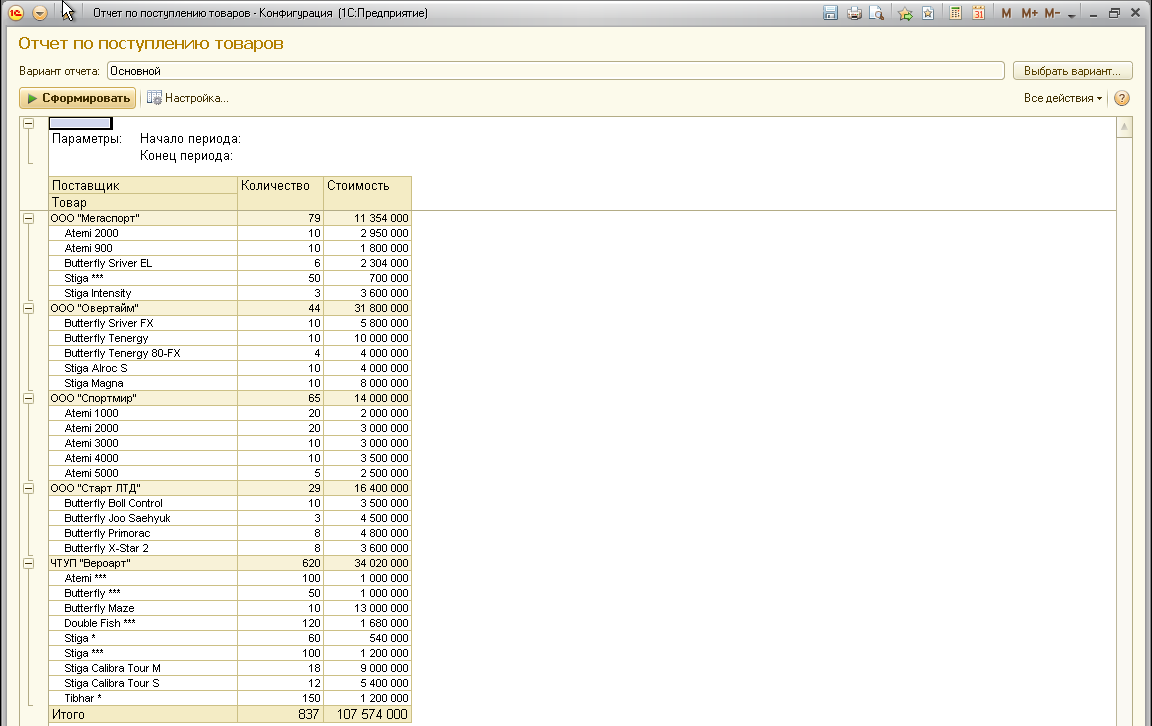
\includegraphics[width=150mm]{pic/report_input}
  \caption{Отчет <<ОтчетПоПоступлениюТоваров>>}
  \label{fig:report_input}
\end{figure}


%% Реализация товаров
Подобным образом создадим отчет о реализации товаров,
содержащий данные о реализованных товарах, их количествах и стоимости.
Для этого в режиме конфигуратора СКД 1С:Предприятие создадим отчет
<<ОтчетПоРеализацииТоваров>>, с помощью конструктора запросов
определим набор данных, извлекаемых из информационной системы:
<<КоличествоТовараОстаткиИОбороты.Товар>>,
<<КоличествоТовараОстаткиИОбороты.КоличествоРасход>>,
<<КоличествоТовараОстаткиИОбороты.СтоимостьРасход>>,
как показано на рисунке~\ref{fig:report_output_query}.

Схема компоновки данных отчета примет вид,
показанный на рисунке~\ref{fig:report_output_scheme}.

\begin{figure}[h!]
  \centering
  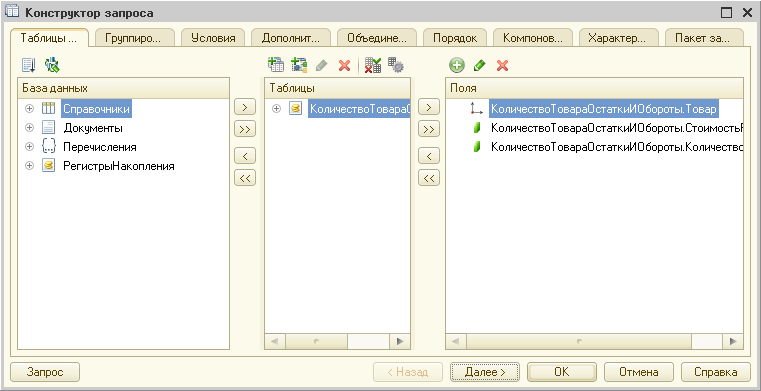
\includegraphics[width=150mm]{pic/report_output_query}
  \caption{Конструктор запросов отчета \\ <<ОтчетПоРеализацииТоваров>>}
  \label{fig:report_output_query}
\end{figure}

\begin{figure}[h!]
  \centering
  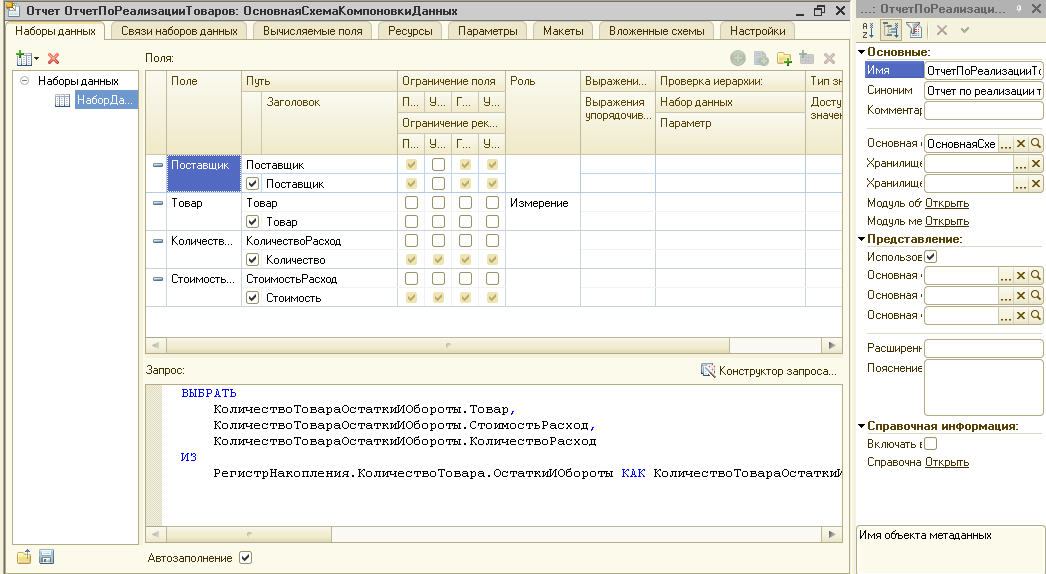
\includegraphics[width=150mm]{pic/report_output_scheme}
  \caption{Схема компоновки данных отчета \\ <<ОтчетПоРеализацииТоваров>>}
  \label{fig:report_output_scheme}
\end{figure}

С помощью конструктора настроек отчета выберем желаемый способ отображения
отчета:
\begin{itemize}
\item тип отчета: список;
\item отображаемые поля: <<Товар>>,
  <<КоличествоРасход>>, <<СтоимостьРасход>>;
\item поля упорядочивания:
  <<СтоимостьРасход>> (по убыванию).
\end{itemize}

Пример разработанного отчета приведен на рисунке~\ref{fig:report_output}.

\begin{figure}[h!]
  \centering
  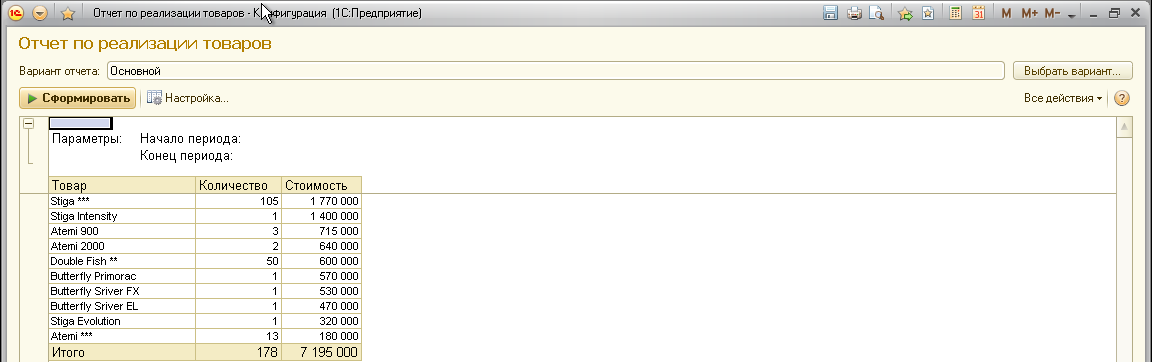
\includegraphics[width=150mm]{pic/report_output}
  \caption{Отчет <<ОтчетПоПоступлениюТоваров>>}
  \label{fig:report_output}
\end{figure}

%% Статистика
Наконец, для отслеживания ассортиментного перечня поставляемых товаров
создадим отчет, содержащий данные о поставщиках,
поступивших товарах, их количествах и стоимости.
Для этого в режиме конфигуратора СКД 1С:Предприятие создадим отчет
<<СтатистикаПоступленияТовара>>, с помощью конструктора запросов
определим набор данных, извлекаемых из информационной системы:
<<КоличествоТовараОстаткиИОбороты.Поставщик>>,
<<КоличествоТовараОстаткиИОбороты.Товар>>,
<<КоличествоТовараОстаткиИОбороты.КоличествоПриход>>,
<<КоличествоТовараОстаткиИОбороты.СтоимостьПриход>>,
как показано на рисунке~\ref{fig:report_stats_query}.

Схема компоновки данных отчета примет вид,
показанный на рисунке~\ref{fig:report_stats_scheme}.

С помощью конструктора настроек отчета выберем желаемый способ отображения
отчета:
\begin{itemize}
\item тип отчета: диаграмма;
\item отображаемые поля: <<Поставщик>>,
  <<Товар>>, <<КоличествоПриход>>;
\item серии: <<Товар>>;
\item точки: <<Поставщик>>;
\item поля упорядочивания:
  <<Поставщик>> (по возрастанию);
\item тип гистограммы:
  <<Гистограмма объемная>>.
\end{itemize}

Пример разработанного отчета приведен на рисунке~\ref{fig:report_stats}.

\begin{figure}[h!]
  \centering
  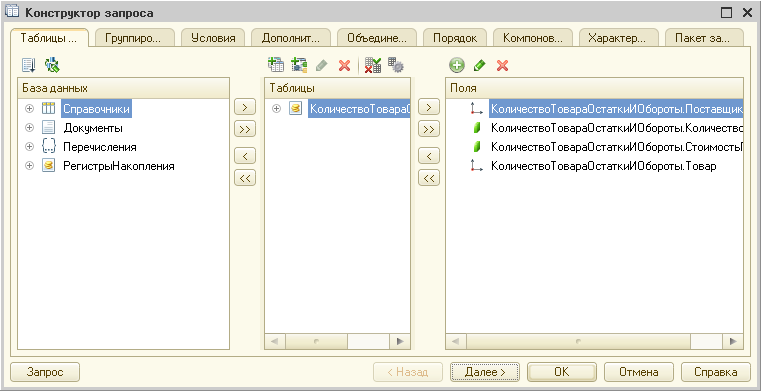
\includegraphics[width=110mm]{pic/report_stats_query}
  \caption{Конструктор запросов отчета \\ <<СтатистикаПоступленияТовара>>}
  \label{fig:report_stats_query}
\end{figure}

\begin{figure}[h!]
  \centering
  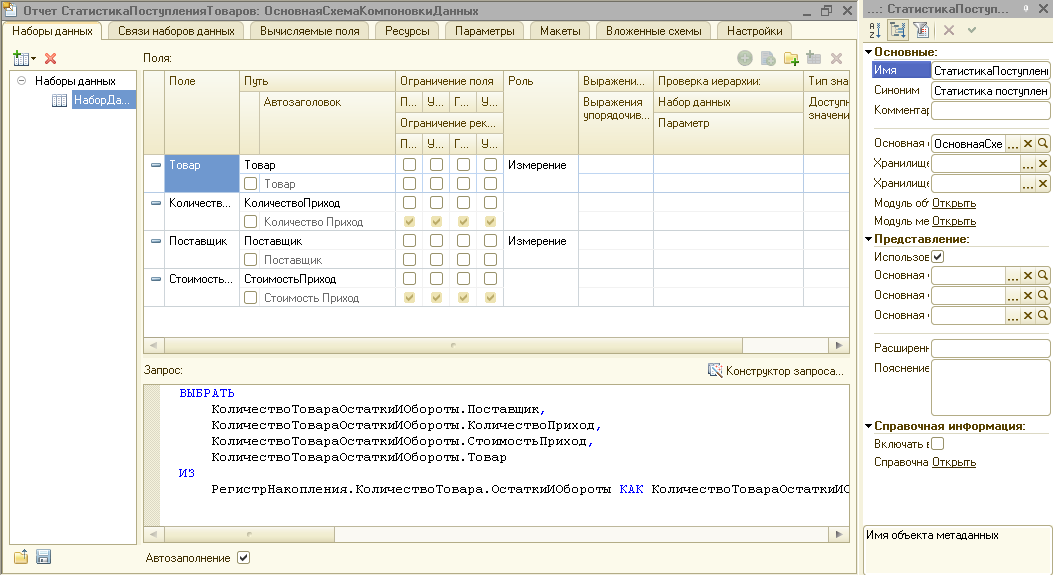
\includegraphics[width=110mm]{pic/report_stats_scheme}
  \caption{Схема компоновки данных отчета \\ <<СтатистикаПоступленияТовара>>}
  \label{fig:report_stats_scheme}
\end{figure}

\begin{figure}[h!]
  \centering
  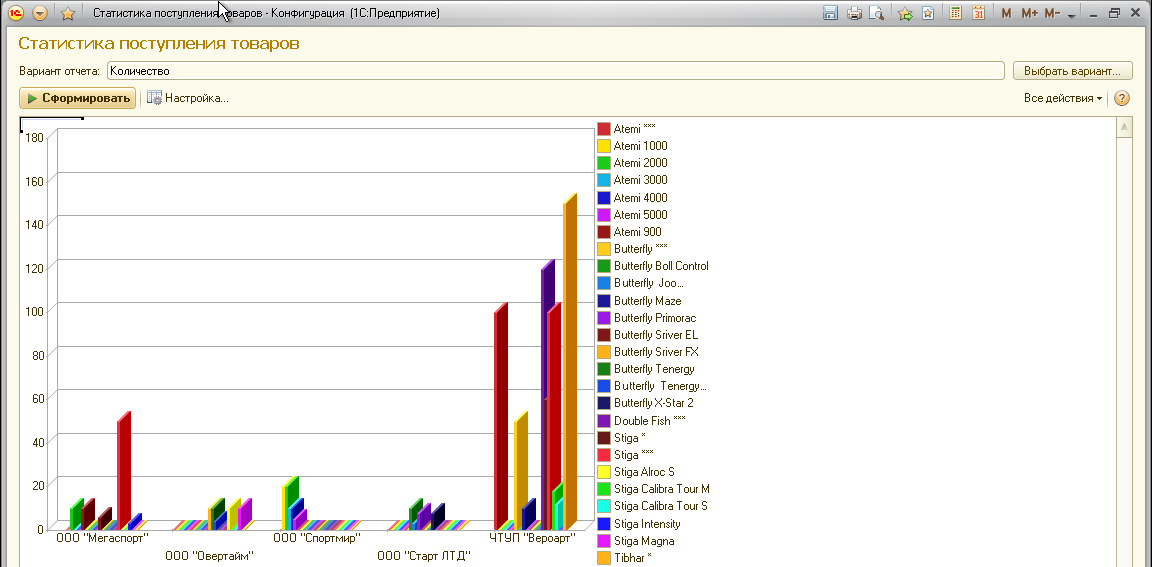
\includegraphics[width=110mm]{pic/report_stats}
  \caption{Отчет <<СтатистикаПоступленияТовара>>}
  \label{fig:report_stats}
\end{figure}

\pagebreak

\subsection{Создание запросов}

Для демонстрации работы запросов в СКД 1С:Предприятие будем
использовать обработки.
Создание обработки производится с помощью раздела
<<Обработки>> панели <<Конфигурация>> режима <<Конфигуратор>>.
Для создания обработки необходимо,
щелкнув правой кнопкой мыши по этому
разделу, выбрать пункт <<Добавить>>. Далее в появившемся окне
следует определить имя и синоним обработки;
на вкладке <<Формы>> создать и настроить форму обработки,
установив требуемые элементы управления, затем на вкладке
<<Модуль>> ввести программный код.

% ДорогиеТоварыЗаданногоПоставщика

Создадим запрос, отображающий три наиболее дорогих товара,
поставленных выбранным поставщиком.
Для этого создадим обработку <<ДорогиеТоварыЗаданногоПоставщика>>
с дополнительным реквизитом <<ВводПоставщика>> и командой
<<ВыбратьДанные>>, как показано на рисунке~\ref{fig:query_most_form}.

На вкладке <<Модуль>> формы назначим обработчик нажатия кнопки
<<ВыбратьДанные>>, как показано на рисунке~\ref{fig:query_most_module}.

На рисунке~\ref{fig:query_most_result} приведен результат
выполнения обработки.

\begin{figure}[h!]
  \centering
  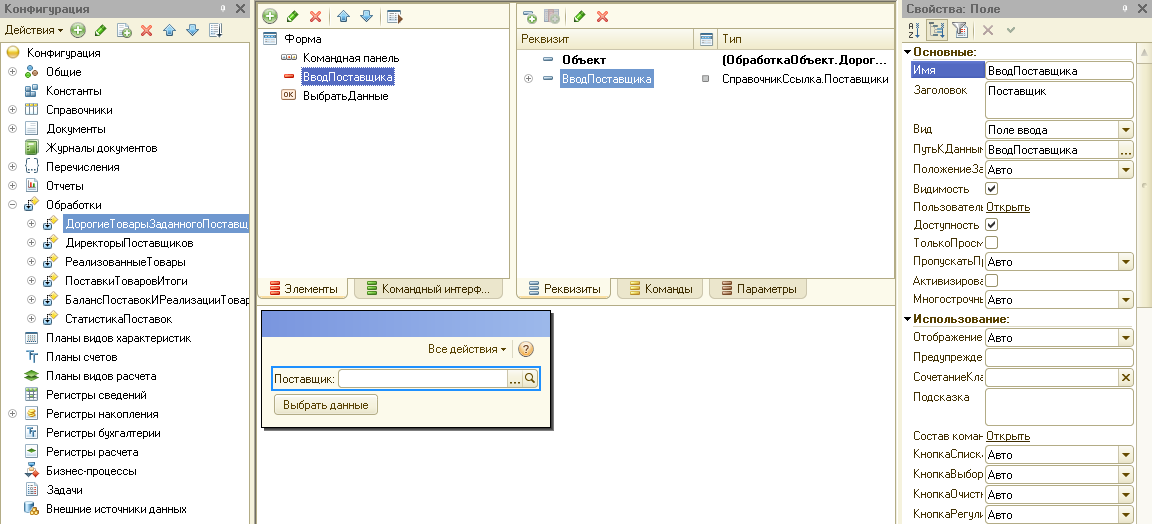
\includegraphics[width=150mm]{pic/query_most_form}
  \caption{Форма обработки <<ДорогиеТоварыЗаданногоПоставщика>>}
  \label{fig:query_most_form}
\end{figure}

\begin{figure}[h!]
  \centering
  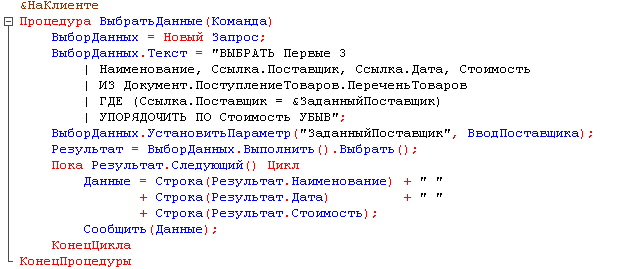
\includegraphics[width=130mm]{pic/query_most_module}
  \caption{Модуль формы обработки \\ <<ДорогиеТоварыЗаданногоПоставщика>>}
  \label{fig:query_most_module}
\end{figure}

\begin{figure}[h!]
  \centering
  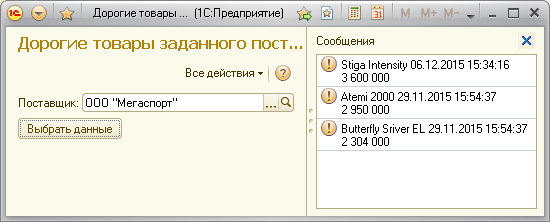
\includegraphics[width=150mm]{pic/query_most_result}
  \caption{Результат выполнения обработки \\ <<ДорогиеТоварыЗаданногоПоставщика>>}
  \label{fig:query_most_result}
\end{figure}

\pagebreak
% ДиректорыПоставщиков

Создадим запрос, отображающий информацию (предприятие, ФИО и номер телефона),
всех директоров предприятий-поставщиков.
Для этого создадим обработку <<ДиректорыПоставщиков>>
с командой <<ВыбратьДанные>>,
как показано на рисунке~\ref{fig:query_directors_form}.

На вкладке <<Модуль>> формы назначим обработчик нажатия кнопки
<<ВыбратьДанные>>, как показано на рисунке~\ref{fig:query_directors_module}.

На рисунке~\ref{fig:query_directors_result} приведен результат
выполнения обработки.

\begin{figure}[h!]
  \centering
  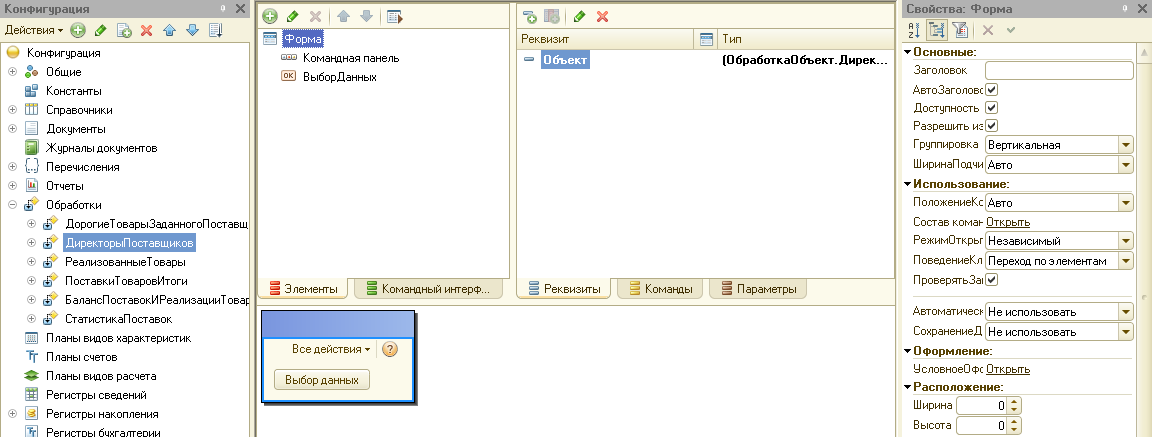
\includegraphics[width=130mm]{pic/query_directors_form}
  \caption{Форма обработки <<ДиректорыПоставщиков>>}
  \label{fig:query_directors_form}
\end{figure}

\begin{figure}[h!]
  \centering
  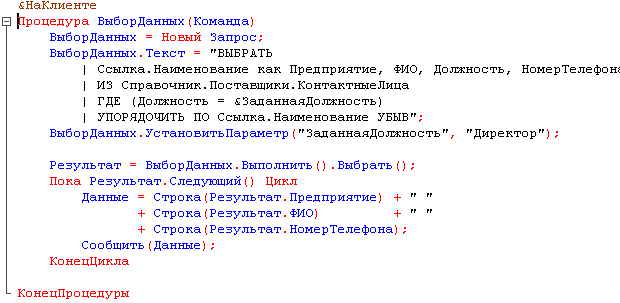
\includegraphics[width=130mm]{pic/query_directors_module}
  \caption{Модуль формы обработки \\ <<ДиректорыПоставщиков>>}
  \label{fig:query_directors_module}
\end{figure}

\begin{figure}[h!]
  \centering
  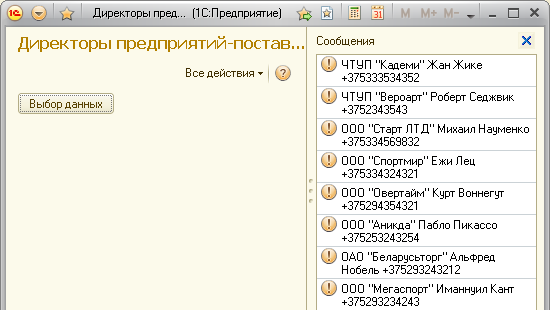
\includegraphics[width=110mm]{pic/query_directors_result}
  \caption{Результат выполнения обработки \\ <<ДиректорыПоставщиков>>}
  \label{fig:query_directors_result}
\end{figure}

\pagebreak
% РеализованныеТовары

Создадим запрос, отображающий список реализованных товаров,
их суммарной стоимостью и количеством, сгруппированных по
наименованию, с не менее чем указанной стоимостью.
Для этого создадим обработку <<РеализованныеТовары>>
с дополнительным реквизитом <<ВводМинимальнойСтоимости>> и
командой <<ВыбратьДанные>>,
как показано на рисунке~\ref{fig:query_output_form}.

На вкладке <<Модуль>> формы назначим обработчик нажатия кнопки
<<ВыбратьДанные>>, как показано на рисунке~\ref{fig:query_output_module}.

На рисунке~\ref{fig:query_output_result} приведен результат
выполнения обработки.

\begin{figure}[h!]
  \centering
  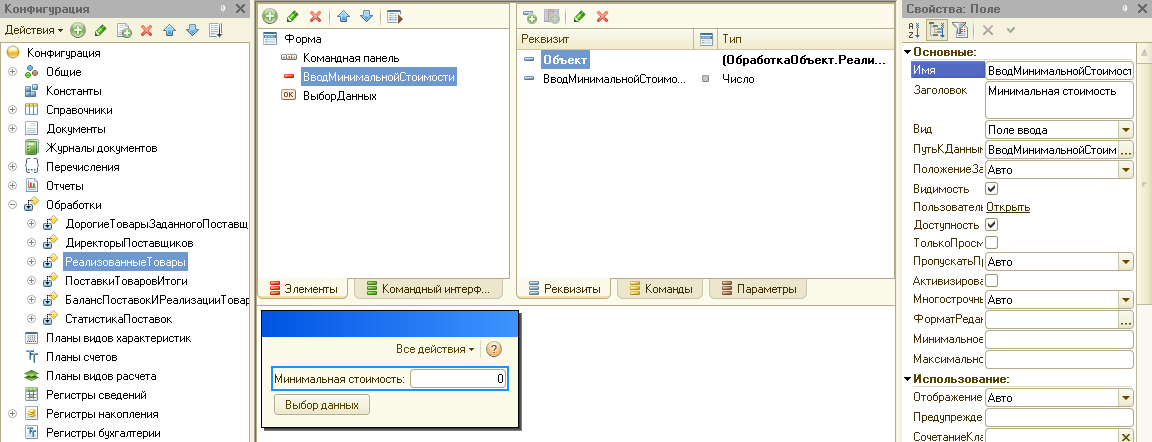
\includegraphics[width=150mm]{pic/query_output_form}
  \caption{Форма обработки <<РеализованныеТовары>>}
  \label{fig:query_output_form}
\end{figure}

\begin{figure}[h!]
  \centering
  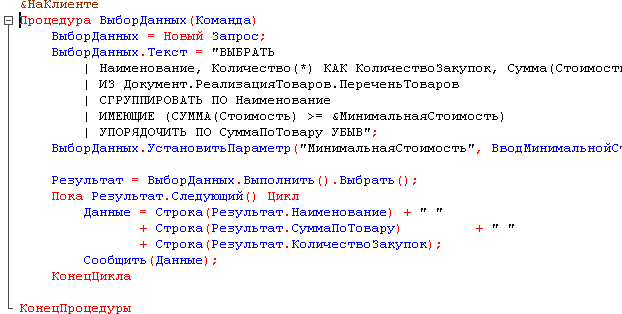
\includegraphics[width=130mm]{pic/query_output_module}
  \caption{Модуль формы обработки \\ <<РеализованныеТовары>>}
  \label{fig:query_output_module}
\end{figure}

\begin{figure}[h!]
  \centering
  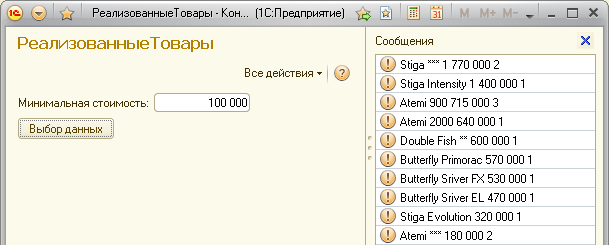
\includegraphics[width=150mm]{pic/query_output_result}
  \caption{Результат выполнения обработки \\ <<РеализованныеТовары>>}
  \label{fig:query_output_result}
\end{figure}

\pagebreak
% ПоставкиТоваровИтоги

Создадим запрос, отображающий информацию о поставках товаров:
поставщике, наименовании, количестве и стоимости товаров с итоговвыми
значениями суммы и количества товаров по каждому поставщику
и наименованию товара.
Для этого создадим обработку <<ПоставкиТоваровИтоги>>
с командой <<ВыбратьДанные>>,
как показано на рисунке~\ref{fig:query_input_form}.

На вкладке <<Модуль>> формы назначим обработчик нажатия кнопки
<<ВыбратьДанные>>, как показано на рисунке~\ref{fig:query_input_module}.

На рисунке~\ref{fig:query_input_result} приведен результат
выполнения обработки.

\begin{figure}[h!]
  \centering
  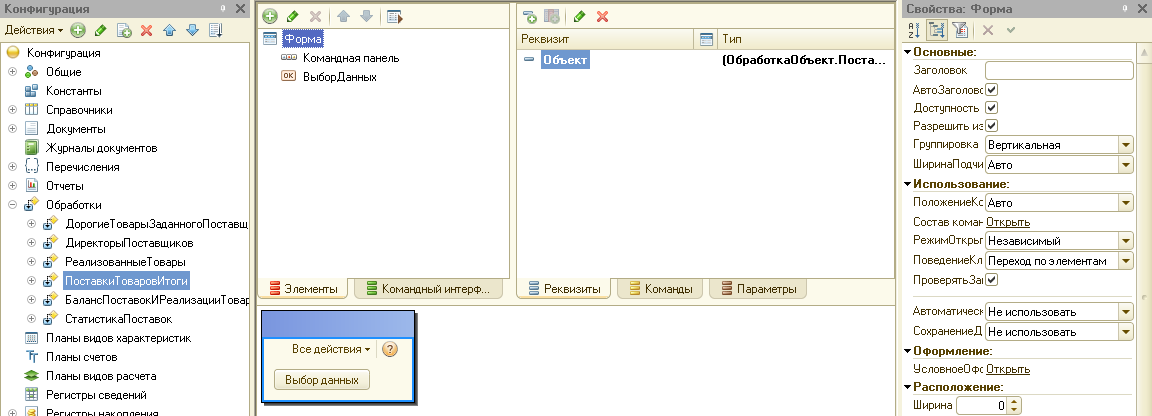
\includegraphics[width=150mm]{pic/query_input_form}
  \caption{Форма обработки <<ПоставкиТоваровИтоги>>}
  \label{fig:query_input_form}
\end{figure}

\begin{figure}[h!]
  \centering
  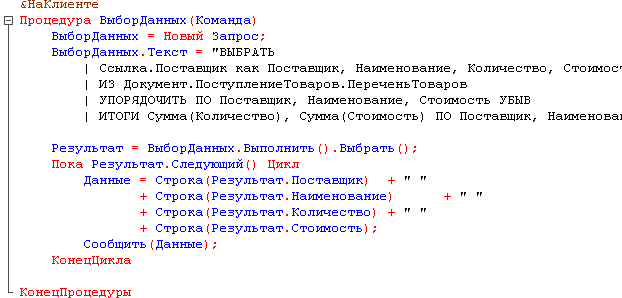
\includegraphics[width=130mm]{pic/query_input_module}
  \caption{Модуль формы обработки \\ <<ПоставкиТоваровИтоги>>}
  \label{fig:query_input_module}
\end{figure}

\begin{figure}[h!]
  \centering
  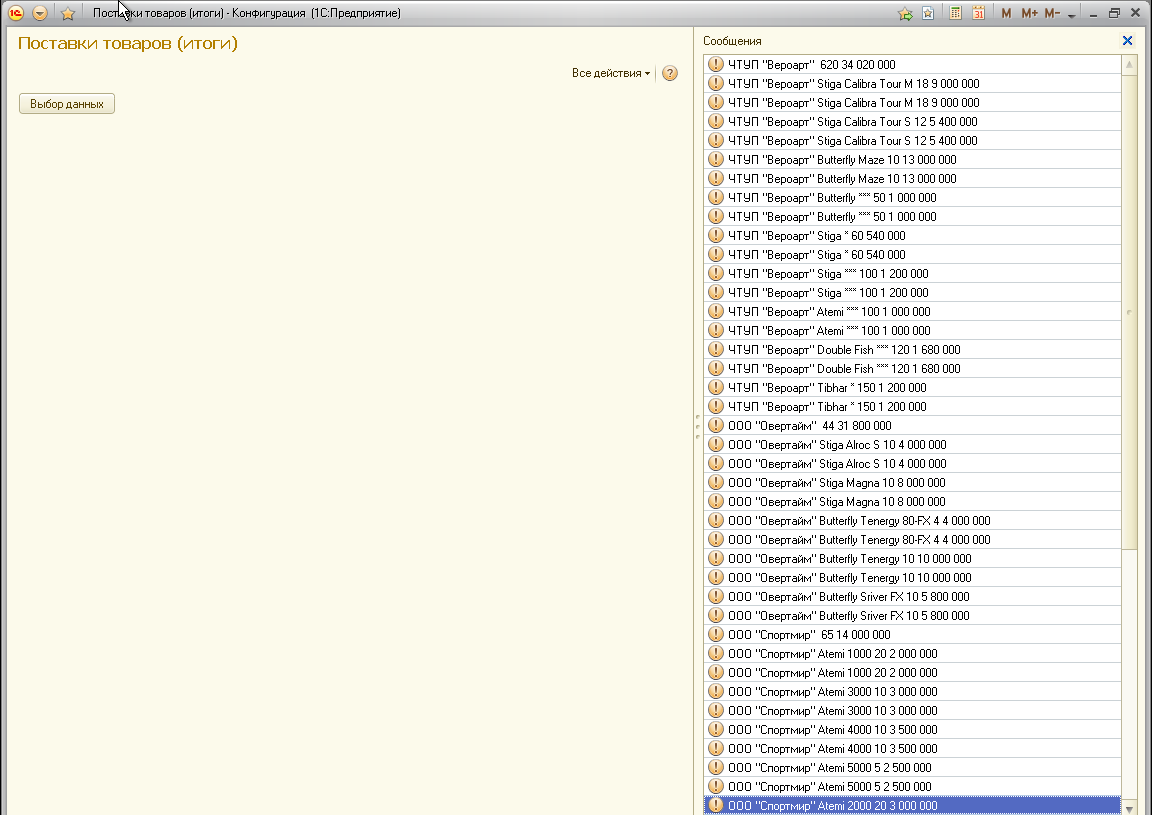
\includegraphics[width=150mm]{pic/query_input_result}
  \caption{Результат выполнения обработки \\ <<ПоставкиТоваровИтоги>>}
  \label{fig:query_input_result}
\end{figure}

\pagebreak
% БалансПоставокИРеализацииТоваров

Создадим запрос, отображающий баланс между общей стоимостью поставок и
реализации по каждому наименованию товара в виде отчета.
Для этого создадим обработку <<БалансПоставокИРеализацииТоваров>>
с командой <<ВыбратьДанные>>,
как показано на рисунке~\ref{fig:query_balance_form}.

Для отображения результатов выполнения запроса в отчете,
создадим макет отчета с помощью раздела <<Макеты>> обработки
<<БалансПоставокИРеализацииТоваров>>.
Определим в нем разделы <<Заголовок>>, <<Шапка>> и <<СтрокаОтчета>>,
а также параметры <<НаименованиеТовара>>, <<ОбъемПоступления>> и
<<ОбъемРеализации>>, как показано на рисунке~\ref{fig:query_balance_report}.

На вкладке <<Модуль>> формы обработки назначим обработчик нажатия кнопки
<<ВыбратьДанные>>, как показано на рисунке~\ref{fig:query_balance_module}.

На рисунке~\ref{fig:query_balance_result} приведен результат
выполнения обработки.

\begin{figure}[h!]
  \centering
  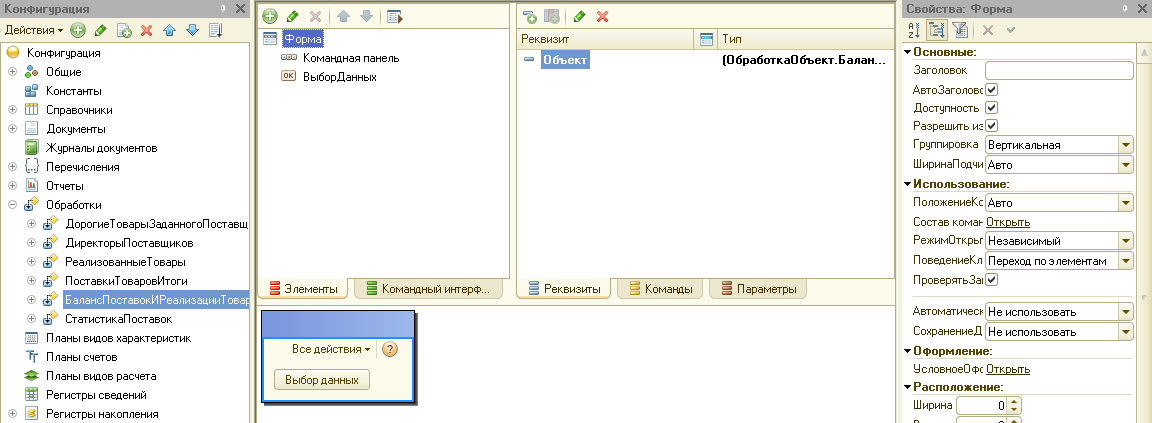
\includegraphics[width=150mm]{pic/query_balance_form}
  \caption{Форма обработки <<БалансПоставокИРеализацииТоваров>>}
  \label{fig:query_balance_form}
\end{figure}

\begin{figure}[h!]
  \centering
  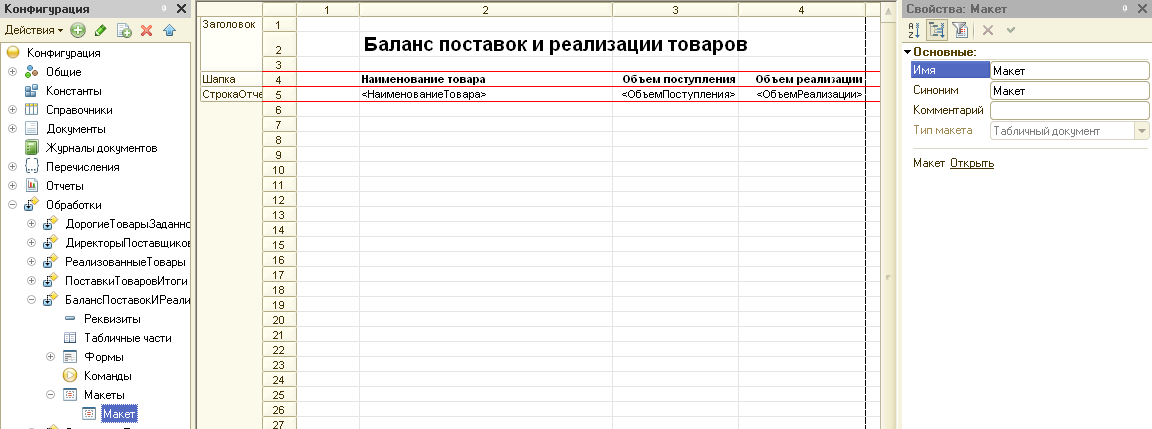
\includegraphics[width=150mm]{pic/query_balance_report}
  \caption{Макет отчета обработки <<БалансПоставокИРеализацииТоваров>>}
  \label{fig:query_balance_report}
\end{figure}

\begin{figure}[h!]
  \centering
  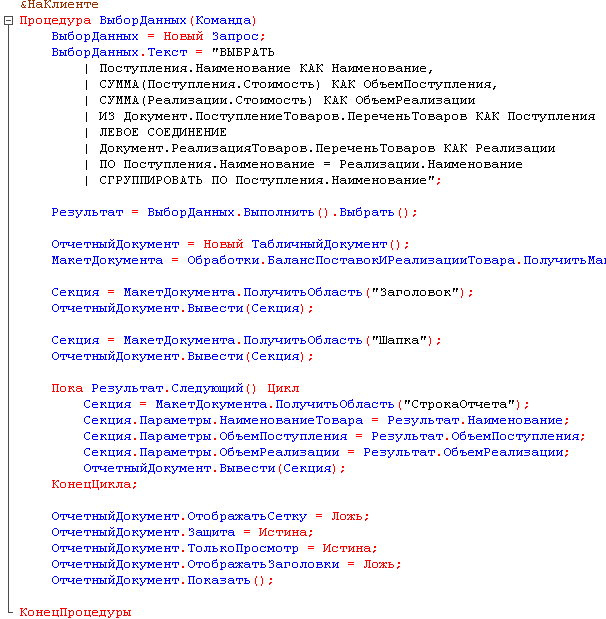
\includegraphics[width=110mm]{pic/query_balance_module}
  \caption{Модуль формы обработки \\ <<БалансПоставокИРеализацииТоваров>>}
  \label{fig:query_balance_module}
\end{figure}

\begin{figure}[h!]
  \centering
  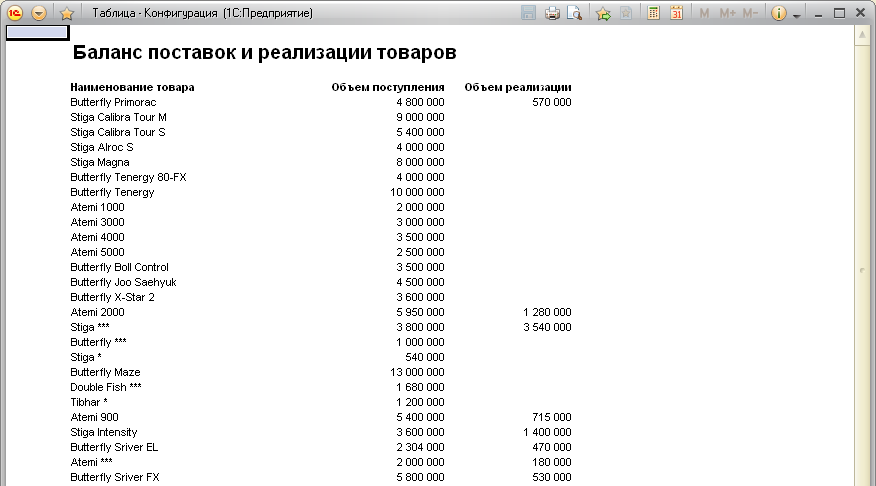
\includegraphics[width=150mm]{pic/query_balance_result}
  \caption{Результат выполнения обработки \\
    <<БалансПоставокИРеализацииТоваров>>}
  \label{fig:query_balance_result}
\end{figure}

\pagebreak
% СтатистикаПоставок

Создадим запрос, отображающий текущее количество товаров на складе,
сгрупированного по поставщикам, в виде отчета.
Для этого создадим обработку <<СтатистикаПоставок>>
с командой <<ВыбратьДанные>>,
как показано на рисунке~\ref{fig:query_input_stats_form}.

Для отображения результатов выполнения запроса в отчете,
создадим макет отчета с помощью раздела <<Макеты>> обработки
<<СтатистикаПоставок>>.
Определим в нем разделы <<Заголовок>>, <<Шапка>> и <<СтрокаОтчета>>,
а также параметры <<НаименованиеПоставщика>>, <<КоличествоТовара>> и
<<СтоимостьТовара>>, как показано на рисунке~\ref{fig:query_input_stats_report}.

На вкладке <<Модуль>> формы обработки назначим обработчик нажатия кнопки
<<ВыбратьДанные>>, как показано на рисунке~\ref{fig:query_input_stats_module}.

На рисунке~\ref{fig:query_input_stats_result} приведен результат
выполнения обработки.

\begin{figure}[h!]
  \centering
  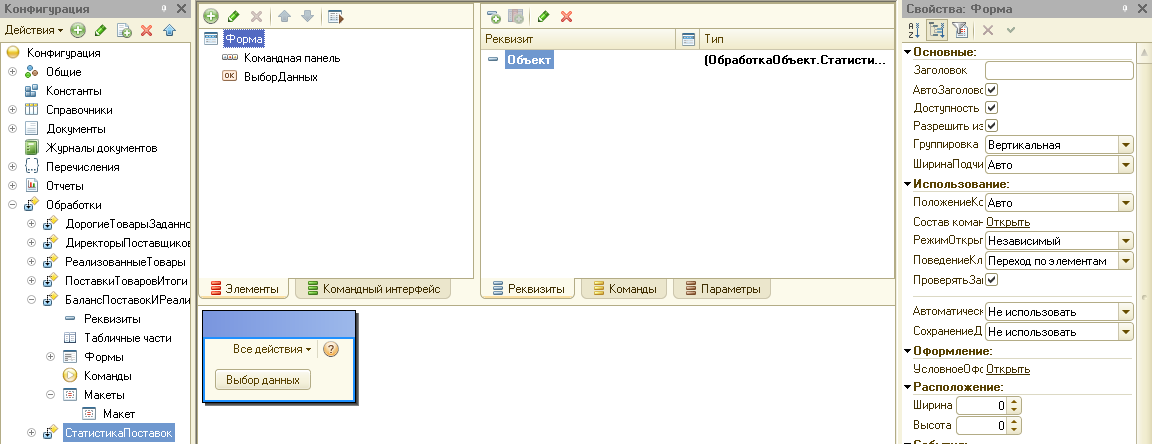
\includegraphics[width=150mm]{pic/query_input_stats_form}
  \caption{Форма обработки <<СтатистикаПоставок>>}
  \label{fig:query_input_stats_form}
\end{figure}

\begin{figure}[h!]
  \centering
  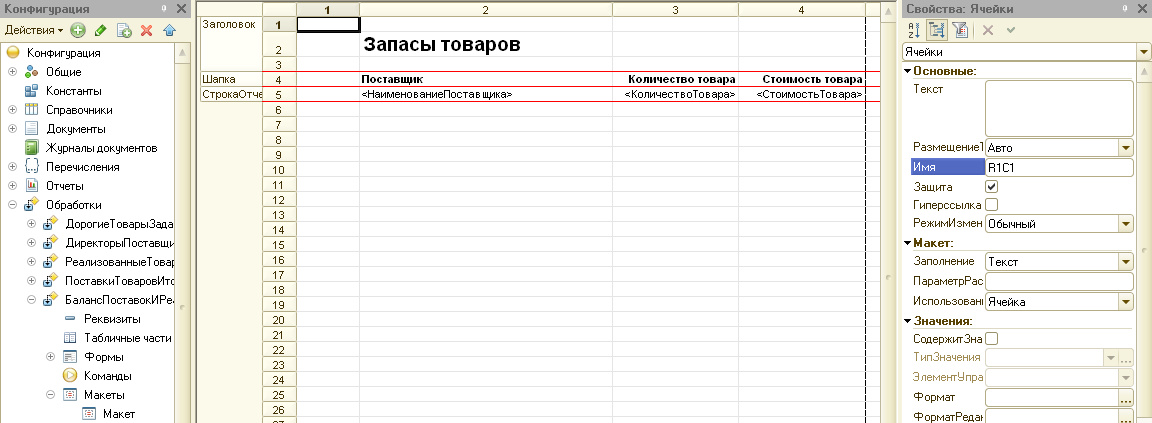
\includegraphics[width=150mm]{pic/query_input_stats_report}
  \caption{Макет отчета обработки <<СтатистикаПоставок>>}
  \label{fig:query_input_stats_report}
\end{figure}

\begin{figure}[h!]
  \centering
  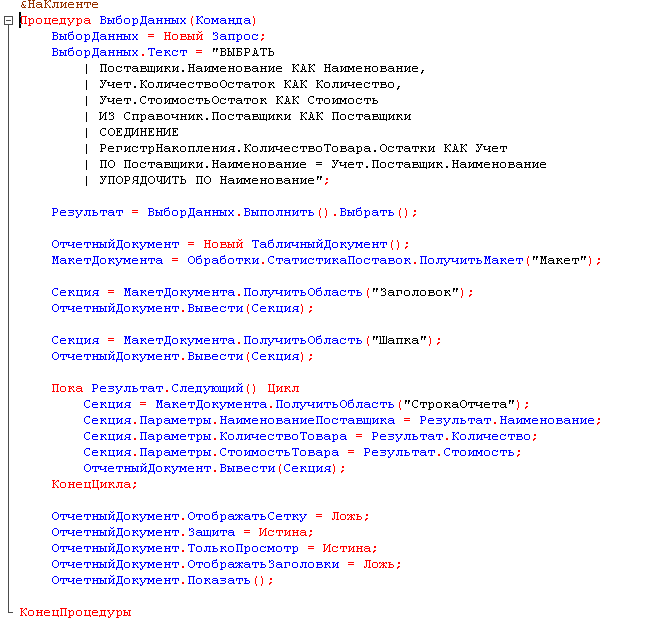
\includegraphics[width=130mm]{pic/query_input_stats_module}
  \caption{Модуль формы обработки \\ <<СтатистикаПоставок>>}
  \label{fig:query_input_stats_module}
\end{figure}

\begin{figure}[h!]
  \centering
  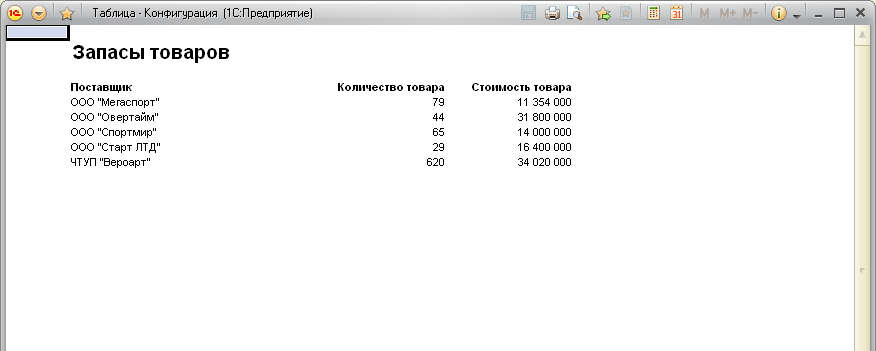
\includegraphics[width=150mm]{pic/query_input_stats_result}
  \caption{Результат выполнения обработки \\
    <<СтатистикаПоставок>>}
  \label{fig:query_input_stats_result}
\end{figure}
